\chapter{Mô hình phân loại điện tâm đồ }
\newpage

\section{Sơ đồ hệ thống phân loại điện tâm đồ}
\begin{center}
    
\includegraphics[scale=.5]{image/chapter5/system.png}
    \begin{figure}[htp]
    \begin{center}
    \end{center}
    \caption{Sơ đồ hệ thống phân loại điện tâm đồ}
    \end{figure}
\end{center}

\section{Tiền xử lý dữ liệu}
Tín hiệu điện tâm đồ khi được thu nhận từ các thiết bị đo ban đầu có khả năng rất cao bị nhiễu do nhiều yếu tố khác nhau, như nhiễu do ảnh hưởng từ cơ bắp, nhiễu sinh ra từ các thiết bị điện tử, nhiễu từ các điện cực của thiết bị đo điện tâm đồ, power line interference, baseline wander,… Nhiễu có tác động rất lớn đến chất lượng của việc trích xuất đặc trưng và do đó ảnh hưởng đến kết quả bài toán phân loại (việc trích xuất đặc trưng từ tín hiệu điện tâm đồ có thể không chính xác và do đó có thể dẫn đến kết quả phân loại, chẩn đoán bị sai). Vì vậy, tín hiệu điện tâm đồ được thu nhận lúc ban đầu cần phải được khử nhiễu trước khi được thực hiện các bước trích xuất đặc trưng và phân loại. Giải pháp cho việc khử nhiễu đó là lọc nhiễu Butterworth bậc 2 gồm high pass, low pass.
\begin{center}
         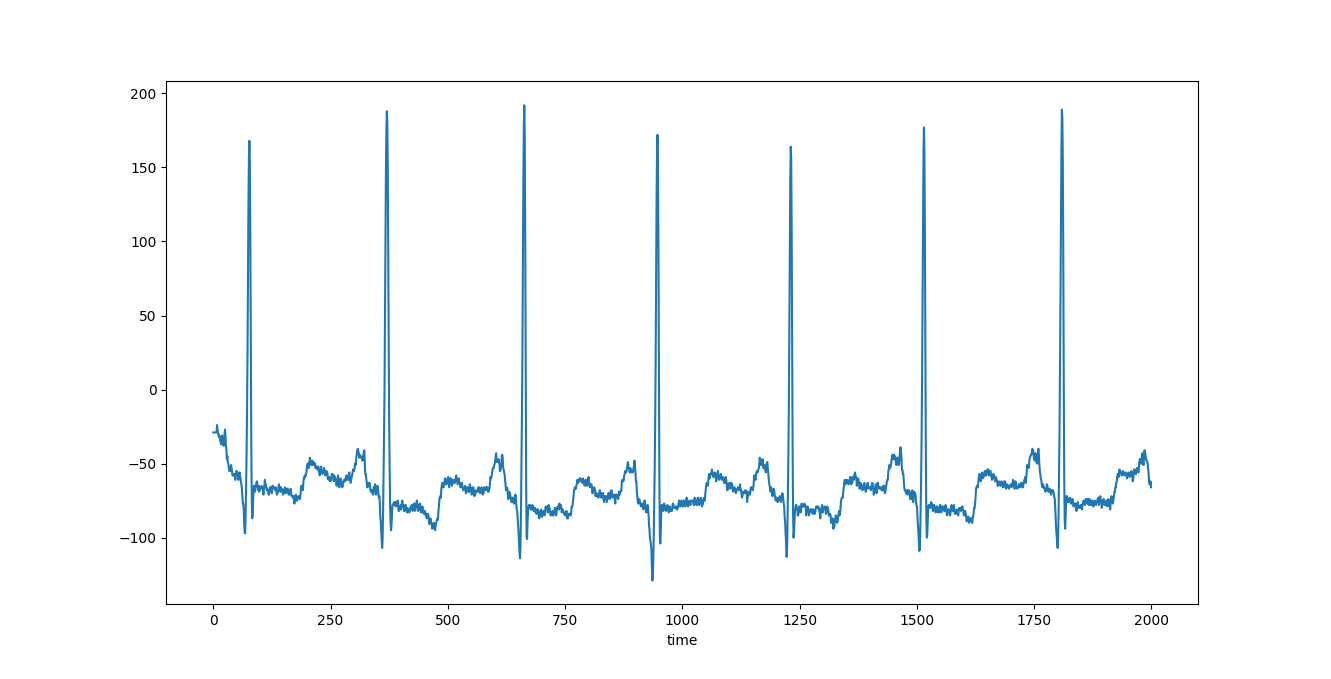
\includegraphics[width=1.\linewidth]{image/chapter5/noise.png}
         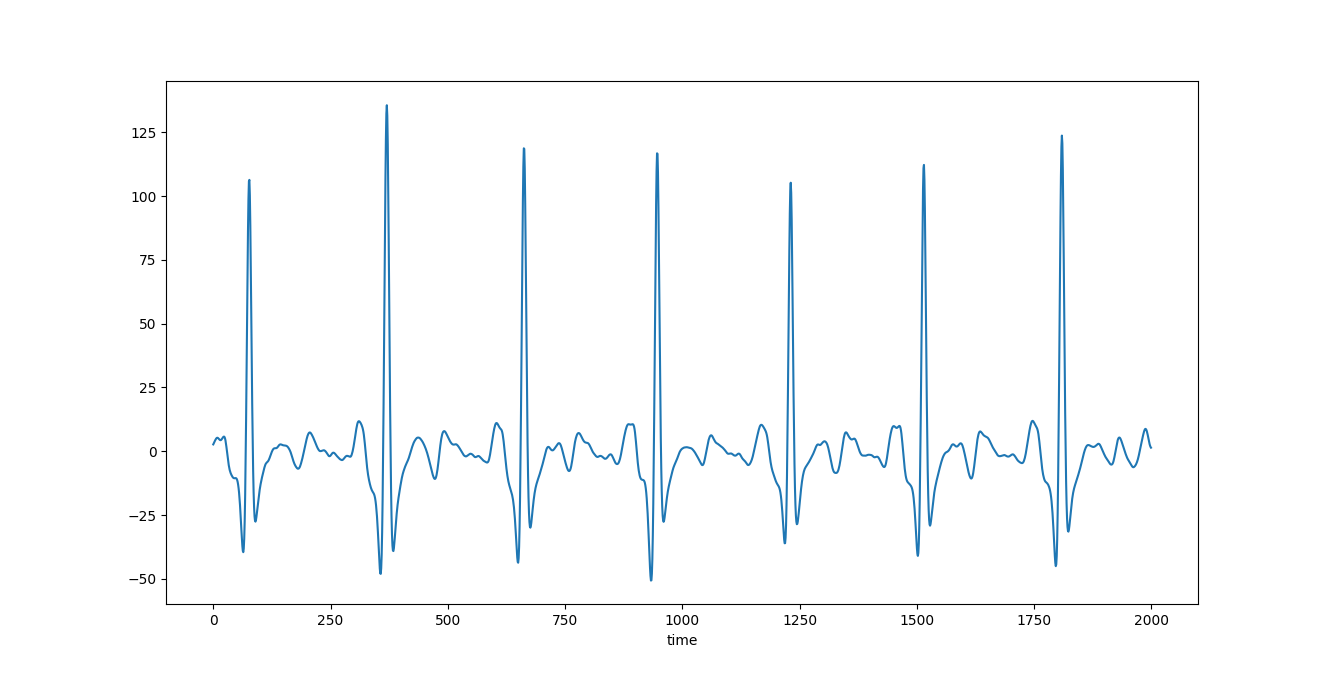
\includegraphics[width=1.\linewidth]{image/chapter5/hlp.png}
    \begin{figure}[!htb]
       \caption{Dữ liệu trước và sau khi lọc nhiễu}
    \end{figure}
\end{center}

\section{Trích xuất đặc trưng}
Dữ liệu sau khi xử lý tiền dữ liệu sẽ được trích xuất đặc trưng bằng kỹ thuật ngưỡng thích ứng kết hợp được đề xuất bới Christov. Những điểm R trong dữ liệu sẽ được đánh nhãn R
\begin{center}
    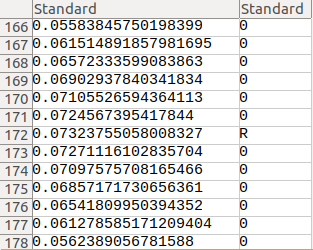
\includegraphics[scale=.5]{image/model/fx_rr.png}
    \begin{figure}[htp]
    \begin{center}
    \end{center}
    \caption{Dữ liệu csv đã được đánh dấu đoạn RR}
    \end{figure}
\end{center}
\begin{center}
    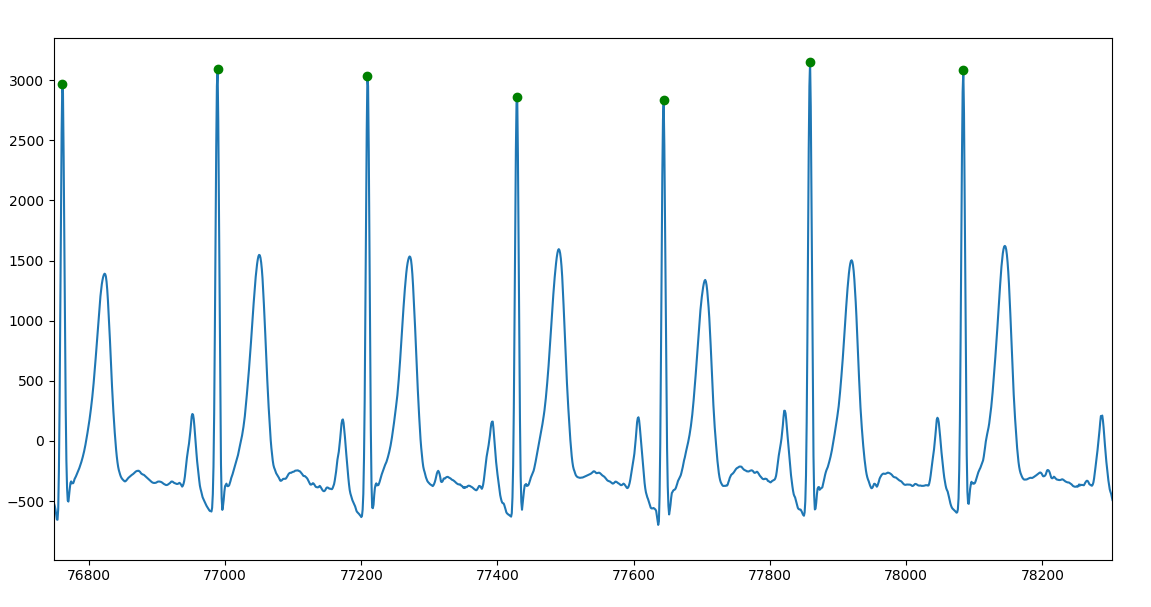
\includegraphics[scale=.4]{image/chapter5/R_detect.png}
    \begin{figure}[htp]
    \begin{center}
    \end{center}
    \caption{Hình ảnh đỉnh R được đánh dấu}
    \end{figure}
\end{center}

\section{Chuẩn hóa đặc trưng độ dài và biên độ khoảng R-R }
Một trong những bước đặc biệt và có ảnh hưởng rất lớn đến chất lượng phân loại tín hiệu điện tâm đồ trong nghiên cứu này là việc chuẩn hóa hình dạng (shape normalization) cho đặc trưng khoảng R-R. Do đặc điểm sinh lý của tim mà các khoảng R-R thường có độ dài khác nhau (nhịp đập của tim thường không bất biến mà sẽ có một sự chênh lệch nhất định). Ở người bình thường, không mắc các bệnh lý về tim mạch, khoảng R-R sẽ dao động trong khoảng 600 – 1200 ms \cite{64} . Sự chênh lệch này tuy không lớn về mặt sinh học nhưng sẽ ảnh hưởng rất lớn đến chất lượng của bài toán phân loại tín hiệu điện tâm đồ. Chỉ một sự thay đổi nhỏ (thậm chí rất nhỏ) về hình dạng khoảng R-R, ví dụ giữa hai đỉnh R có chênh lệch một khoảng nhỏ (ví dụ: 0.01 s), sẽ cho ra một dữ liệu huấn luyện hoàn toàn mới cho bài toán phân loại điện tâm đồ và càng nhiều khoảng R-R có hình dạng dài ngắn khác nhau thì tập dữ liệu huấn luyện được sinh ra sẽ vô cùng lớn. Nếu sự không đồng nhất về mặt hình dạng của các khoảng R-R này không được giải quyết hiệu quả thì việc phân loại những tín hiệu điện tâm đồ mới, không có trong tập dữ liệu huấn luyện, sẽ gặp khó khăn và có thể dẫn đến kết quả phân loại, chẩn đoán không còn chính xác (trường hợp này được gọi là overfit – mô hình phân loại chỉ đáp ứng tốt với dữ liệu huấn luyện mà không còn đáp ứng tốt với dữ liệu kiểm thử hoàn toàn mới). Đó là lý do vì sao các khoảng R-R cần phải được chuẩn hóa về một hình dạng nhất định. Massagram và nhóm nghiên cứu \cite{67}, Bhola và nhóm nghiên cứu đều cho rằng 880 – 900 ms là khoảng thời gian phổ biến nhất của khoảng R-R \cite{68}. Do đó, toàn bộ khoảng R-R trong nghiên cứu này sẽ được chuẩn hóa về khoảng thời gian đồng nhất 900 ms bằng phương pháp nội suy tuyến tính (linear interpolation). Hình dạng của khoảng R-R sau khi đã được chuẩn hóa đồng nhất về cùng một khoảng nhất định sẽ gần như không sai lệch quá nhiều so với khoảng R-R ban đầu. Điều này đồng nghĩa với việc mỗi đoạn R-R sẽ có 324 samples dữ liệu.\\
Dữ liệu sau khi chuẩn hóa về mặt thời gian sẽ được chuẩn hóa tiếp theo chiều cao sóng để đưa về khoảng [0,1] để dể dàng cho việc phân loại.

\section{Phân loại tín hiệu điện tâm đồ}
Mô hìn phân loại tín hiệu điện tâm đồ gồm sự kết hợp giữa mạng LSTM và tâng Fully-connected. Trong đó:
\begin{itemize}
    \item Mạng LSTM ở phần đầu của mô hình có chức năng học những đặc trưng tín hiệu điện tâm đồ có dạng Sequence-to-Sequence (Seq2Seq)
    \item Tầng Fully-Connected ở tầng cuối cùng của mô hình có chức năng phân loại dữ liệu đã được huấn luyện ở mạng LSTM trước đó dựa trên 2 nhãn (label) được cung cấp trước đó là “bình thường” (0) và “bất thường” (1)
\end{itemize}
Các tham số của mô hình phân loại:
\begin{itemize}
    \item Tham số tốc độ học (learning rate) là 0.001, giá trị này ảnh hưởng đến tốc độ hội tụ của quá trình huấn luyện.
    \item Số neuron đầu vào là 128, kích thước thu được khi qua mô hình autoencoder.
    \item Số lượng tầng Fully Connected: 2. Số lượng neuron tầng FC1: 20, số lượng neuron tâng FC2: 20 (có kết hợp kỹ thuật dropout).
    \item Hàm biến đổi: softmax.
    \item Hàm lỗi: Mean Square Error.
    \item Sô lớp phân loại tương ứng với 2 nhãn bình thường (0) và bất thường (1)
    \item Các kỹ thuật tránh overfit: Regularization L2, Dropout, khởi tạo trọng số kiểu Xavier.
    \item Phương pháp tối ưu hóa hàm lỗi: bộ tối ưu SGD.
    \item Số lần tính toán (epoch): 2200.
\end{itemize}

\section{Kết quả, Đánh giá và Trở ngại}
\subsection{Thu thập dữ liệu}
Dữ liệu chủ yếu trong nghiên cứu lần này:
\begin{center}
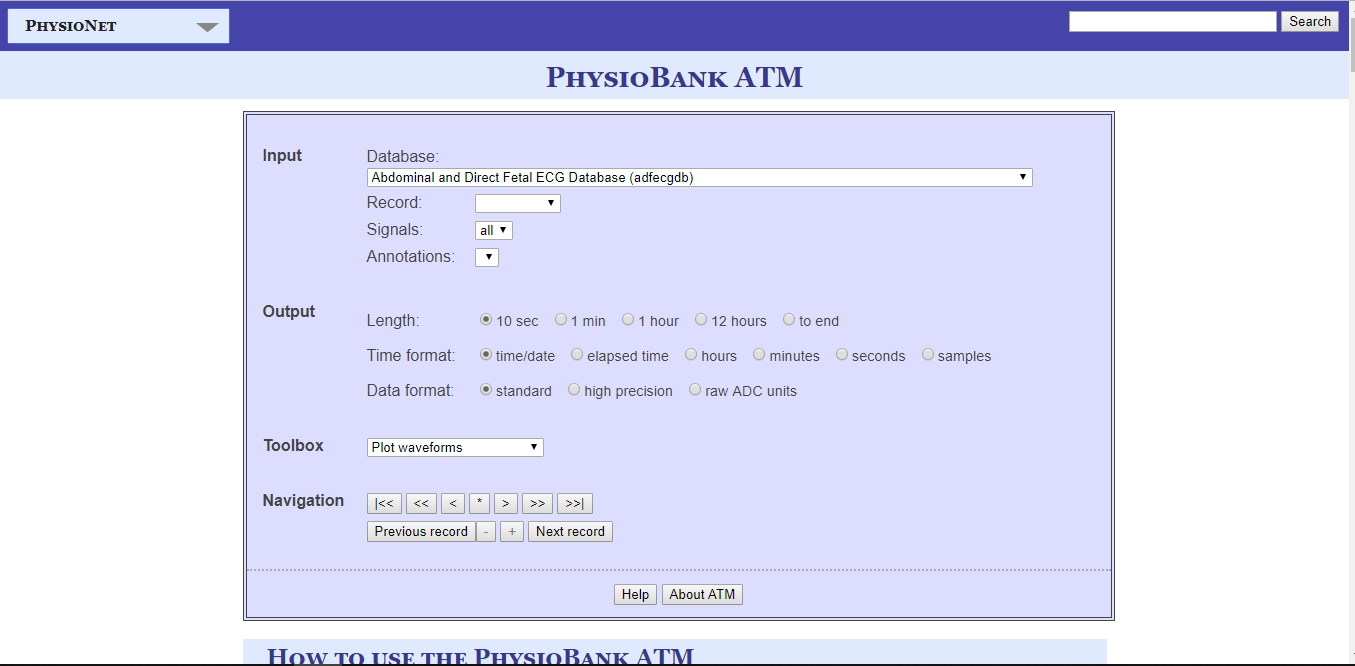
\includegraphics[scale=.3]{image/chapter5/physionet_bank.png}
\begin{figure}[htp]
\begin{center}
\end{center}
\caption{Nguồn thu thập dữ liệu online}
\end{figure}
\end{center}
Bộ dữ liệu được sử dụng: MIT-BIH arrhythmia database.\\
Những đặc điểm của dữ liệu:
\begin{itemize}
    \item Dữ liệu trong thử nghiệm được lấy trên chuyển đạo Lead II trong 2 channel của dữ liệu MIT-BIH vì chuyển đạo này thể hiện rõ ràng nhất đặc điểm của ECG.
    \item Dữ liệu sau khi qua giai đoạn lọc nhiễu và  cắt đoạn RR thu được 98872 (đoạn RR) bao gồm (51765 bình thường và 47107 bất thường)
\end{itemize}
\begin{center}
    \begin{tabular}{|c|c|}
    \hline 
    Tập dữ liệu huấn luyện & Tập dữ liệu kiểm thử \\ 
    \hline 
    79153 & 19719\\ 
    \hline 
    \end{tabular}
\end{center}

\subsection{Kết quả}
Độ chính xác của quá trình phân loại (accuracy): 0.916 và Độ mất mát của quá trình phân loại (loss): 0.052.
\subsection{Đánh giá}
\begin{itemize}
    \item Độ chính xác của mô hình phân loại chưa được cao như những nghiên cứu khác.
\end{itemize}
\subsection{Trở ngoại}
\begin{itemize}
    \item Chỉ mới áp dụng mô hình phân loại trên chuyển đạo Lead II.
    \item Những vấn đề trong việc xử lý dữ liệu, nhiễu...
\end{itemize}

